\section{Firefly-inspired Synchronicity}
\label{sec-algorithm}

In this section, we first describe the Mirollo and Strogatz model and
discuss how the theoretical model differs from practice. Then we
present our modified algorithm, which takes these differences into
account.

\subsection{Mirollo and Strogatz Model}
\label{sec:strogatz}

In the Mirollo and Strogatz (M\&S) model, a node acts as an oscillator
with a fixed time period $T$. Each node has an internal time or phase
$t$, which starts at zero and increments at a constant rate until
$t=T$. At this point the node ``fires'' (in the case of firefly,
flashes) and resets $t=0$. Nodes may start at different times,
therefore their internal time (phase) $t$ is not synchronized.

In the absence of any input from neighbors, a node B simply fires
whenever $t=T$. If B observes a neighbor firing, then B reacts by
adjusting its phase forward, thus shortening its own time to fire
(Figure \ref{fig:firefly-example}(a,b)).

The amount of adjustment is determined by the function $f(t)$, which
is called the {\em firing function}, and the parameter $\epsilon$,
which is a small constant $< 1$. Suppose node B observes a neighbor
fire at $t=t'$. In response, node B {\em instantaneously jumps} to a
new internal time $t = t''$, where

\begin{equation}
\label{eqn:strogatz}
t'' = f^{-1}(f(t') + \epsilon)
\end{equation}

However if $t'' > T$, then $t = T$ and the node immediately fires and
resets $t=0$. In a biological sense, $f(t)$ can be thought of as the
charge of a capacitor within the neuron or firefly, which receives a
boost of $\epsilon$ whenever a firing event is
observed. Algorithmically, the effect is that a node instantaneously
increments its phase by $\Delta(t') = (t'' - t')$, when it observes a
firing event at $t=t'$.

The seminal result by Mirollo and Strogatz is that if the function $f$
is smooth, monotonically increasing, and concave down, then a set of
$n$ nodes will always converge to the same phase (i.e achieve
synchronicity), for any $n$ and any initial starting times
\cite{strogatz}. The simple requirements on $f$ ensure that a node
reacts more strongly to events that occur later in its time
period. One of the limitations of their proof was that it only held
for the case where all $n$ nodes could observe each others' firing
(all-to-all topology). Recently Lucarelli and Wang \cite{lucarelli04}
relaxed this condition and proved that this simple node behavior also
results in synchrony in multi-hop topologies, a prerequisite for use
in sensor networks.

\subsection{From Theory to Practice}

The M\&S model has several salient features. The node algorithm and
the communication are very simple. A node only needs to observe firing
events from neighbors --- there is no strength associated with the
event or even a need to know which neighbor reported the
event. Individual nodes have no state other than their internal
time. Synchronicity provably emerges without any explicit leaders and
irrespective of the starting state.

Because of these reasons, the model is particularly attractive as an
algorithm for sensor networks. However, the theoretical results in
\cite{strogatz,lucarelli04} make several assumptions which are
problematic for wireless sensor networks. These include:

\begin{enumerate}

\item When a node fires, its neighbors instantaneously observe that
event. 

\item Nodes can instantaneously react by firing.

\item Nodes can compute $f$ and $f^{-1}$ perfectly using continuous
mathematics and can compute instantaneously.

\item All nodes have the same time period $T$.

\item Nodes observe all events from their neighbors (no loss).

\end{enumerate}

In a wireless setting, a {\em firing event} can be implemented as a
node sending a broadcast message to its neighbors indicating that it
fired. However, as mentioned before, nodes experience an unpredictable
delay prior to transmission, based on channel contention. Thus, when a
node A sends out a firing event message at time $t$, its neighbor
B will not receive the message until time $t + \delta$ where the
delay $\delta$ is not known in advance.  This violates assumptions 1
and 2. Node B does not know when the actual firing event occurred
and node B can not react instantaneously to node A's behavior. In
addition, the best case for the theoretical model --- i.e. all nodes
fire simultaneously --- constitutes a worst case scenario for channel
contention because it creates the potential for many collisions,
resulting in large message delays.

The other assumptions also pose potential problems, though not quite
as problematic as message delays. Computation accuracy is limited due
to the absence of efficient floating point arithmetic.  Sensor nodes
exhibit slightly different oscillator frequencies. Links between nodes
exhibit varying quality and thus varying levels of message loss. At
the same time, real biological systems are known to have such
variations. Therefore not all of the theoretical assumptions may be
important in practice.

%% Links between nodes are not perfect, not
%% symmetric, and fluctuate over time.  Crystal impurities cause
%% noticeable skew between oscillators.  And the absence of
%% floating-point units on typical sensor network device processors
%% renders floating-point calculations either computationally expensive
%% or impossible.


\subsection{The Reachback Firefly Algorithm (RFA)}

In this paper we focus mainly on the issues related to wireless
communication. We tackle the three problems related to wireless
communication in the following way: (1) We use low level timestamping
to estimate the amount of time a message was delayed before being
broadcast; (2) we modify the node algorithm and introduce the notion
of ``reachback'' in which a node reacts to messages from the previous
time period rather than the current time period, and (3) we
preemptively stagger messages to avoid worst case wireless contention.
Lastly, we use a simple, approximate firing function that can be
computed quickly.

\begin{figure}[t]
\begin{center}
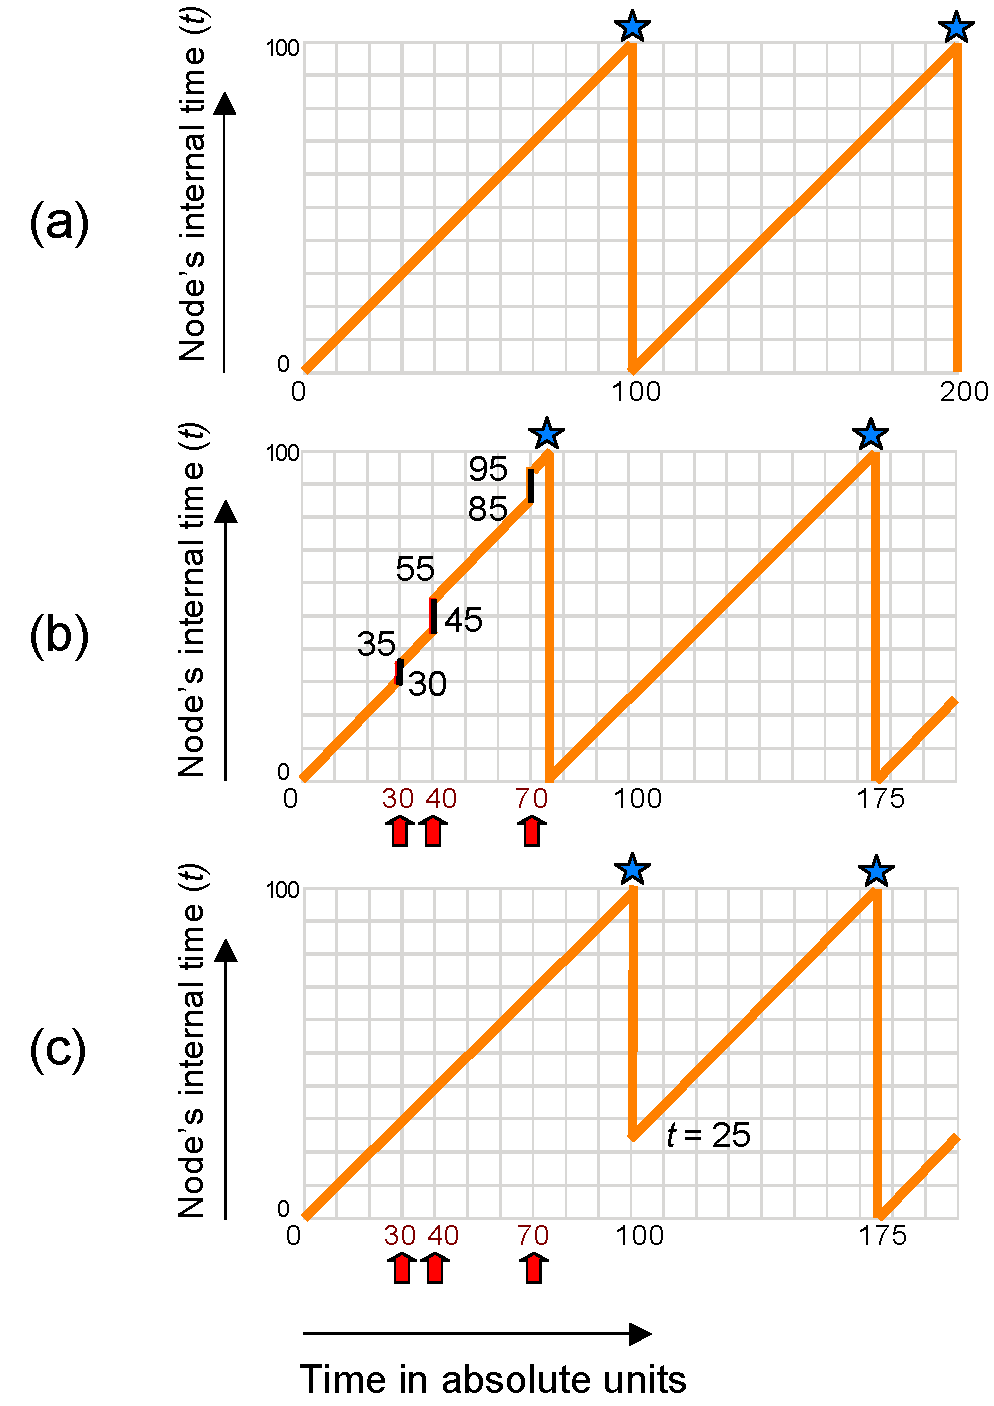
\includegraphics[width=0.8\hsize]{./figures/firing-diagram-cropped.pdf}
\end{center}
\caption{The firefly-inspired node algorithm. (a) A node fires
whenever its internal time $t$ is equal to the default time period $T$
(=100). (b) In the M\&S model, a node responds to neighbors firing
(arrows) by instantaneously incrementing $t$. (c) In RFA, a node
records the firing events and then responds all at once at the
beginning of the next cycle.}
\label{fig:firefly-example}
\end{figure}


{\bf Timestamping Messages.} In order to estimate the delay between
when a node ``fires'' and when the actual message is transmitted, we
use MAC-layer timestamping to record the MAC delay experienced by a
message prior to transmission. The MAC delay can be measured by an
event triggered by the TinyOS radio stack when the message is about to
be transmitted, and is recorded in the header of the outgoing message.
When a node receives a firing message, it uses this information to
determine the correct firing time of the transmitting node by
subtracting the MAC delay from the reception time of the message. This
is very similar to the approach used in time synchronization protocols
such as FTSP~\cite{ftsp} to estimate message transmission delays.

{\bf The {\em Reachback Response.}} The timestamping allows a node B
to correctly identify when a neighbor A fired. However it only
receives this information after some delay, and thus node B can not
react instantaneously to node A's firing.

This causes two problems. First, node B may have already fired and
thus no longer be able to react to node A. This is especially likely
for neighbor firings that occur late in a node's time
period. Furthermore, messages later in the cycle are important and
have a larger adjustment effect (as a result of $f(t)$ being concave
down). Secondly, as a result of the delays, a node may receive firing
messages {\em out of order}. The effect of applying two firing events
is not commutative. Suppose two firings occur at times $t_1$ and $t_2$
($t_1<t_2$). If a node learns of the events out of order, it will
incorrectly advance its phase by $\Delta(t_2) + \Delta(t_1)$ instead
of $\Delta(t_1) + \Delta(t_2 + \Delta(t_1))$. Therefore for the
algorithm to be correct, a node would need to undo and redo the
adjustments, quickly making the algorithm complicated and
unmanageable.

Instead, in order to deal with delayed information, we introduce the
notion of {\em reachback response.} In the reachback response, when a
node hears a neighbor fire, it does not immediately react. Instead, it
places the message in a queue, timestamped with the correct internal
time $t'$ at which the firing event occurred. When the node reaches
time $t=T$, it fires. Then it ``reaches back in time'' by looking at
the queue of messages received during the past period. Based on those
messages, it computes the overall jump and increments $t$ immediately
(Figure \ref{fig:firefly-example}(c)).

The computation is the same as in the M\&S model described in Section
\ref{sec:strogatz}; from the point of view of a node, it is as if it
were receiving firing messages instantaneously. The only difference is
that the messages it is receiving are actually from the {\em previous}
time period. Thus a node is always reacting to information that is one
time period old. In Section {\ref{sec-theory} we present theoretical
results to support why the reachback response still converges. 

%% \begin{figure}[t]
%% \begin{tabular}{lll}
%% $t_{actual}$ &  $t_{internal}$ &  $t_{internal} + {jump}$\\
%% \hline\\
%% 30 & 30 & 30 + \Delta(30) = 35\\
%% 40 & 45 & 45 + \Delta(45) = 55 \\    
%% 70 & 85 & 85 + \Delta(85) = 95 \\
%% \hline\\
%% \end{tabular}
%% \label{table:strogatz}
%% \caption{Computing the effect of neighbors firing, using the Mirollo and Strogatz Model}
%% \end{figure}


{\em Example:} Here we illustrate how the algorithm works through an
example, shown in Figure \ref{fig:firefly-example}. We first
show how the M\&S model works, i.e. when messages are received
instantaneously and the node reacts instantaneously. We then
illustrate the reachback response using the same example.

Let the time period $T = 100$ time units. Let node B start at internal
time $t=0$ and increment $t$ every unit time.  Suppose firing events
arrive at absolute times $30, 40$ and $70$. Let $\Delta(t)$ be some
jump function; here we simply pick jump values for illustration
purposes.

In the M\&S model, the node reacts as each event arrives, by causing
an instantaneous jump in its internal time. $\Delta(t)$ represents the
instantaneous jump at internal time $t$. When node B observes a
firing at time $t=30$, it computes an instantaneous jump of
$\Delta(30)=5$, and sets $t = 30+\Delta(30) = 35$. Ten more time units
from this point on it observes another event. While this event
occurred 40 units of time since the beginning of the cycle, the node
perceives it as having happened at internal time $t = 45$. The node
again computes an instantaneous jump in internal time $t=45+\Delta(45)
= 55$. After 30 more time units the node B observes another firing
event. At this point $t=85$ and the node computes an instantaneous
jump to $t=85+\Delta(85)=95$. After 5 more time units, $t=100$ and
node B fires. 

It is also possible for the computed $t$ to be larger than 100
(e.g. if $\Delta(85)=20$ then $t=85+20=105$), in which case the node
sets $t=100$, immediately fires, and resets $t=0$.

The overall effect is that node B advances its phase (or shortens
its time to fire) by 25 time units. It then continues to fire with the
default time period of $T=100$.

%% THIS IS THE TABLE DATA
%% $t_{actual}$ &  $t_{internal}$ &  $t_{internal} + {jump}$\\
%% 30 & 30 & 30 + \Delta(30) = 35\\
%% 40 & 45 & 45 + \Delta(45) = 55 \\    
%% 70 & 85 & 85 + \Delta(85) = 95 or 105\\

Now we use the same example to illustrate the reachback response. As
before, let node B start with $t=0$ and increment $t$ every time
unit. When node B receives a message, it uses the timestamping
information to determine when that message would have been received
had there been no delay. It then places this information in a queue
and continues.

When $t=100$, node B fires, resets $t=0$, and then looks at the
queue. In this example, the queue contains three events at times 30,
40 and 70. Using the same method described for M\&S, the node computes
how much it would have advanced its phase. Since all of the
information already exists, it can compute the result in one shot.  As
in the previous case, the result is that the phase is advanced by 25
time units. Node B applies this effect by instantaneously jumping from
$t=0$ to $t=25$. It then proceeds as before, firing by default at
$t=100$ if no events are received. The difference between the
reachback scheme and the original M\&S method is that the first firing
event occurs at different absolute times (100 vs 75). This influences
neighboring nodes' behavior and one must prove that the new scheme will
still converge.


%% The queue but it
%% computes using all events within the past 100 time units.  (that is
%% the previous time period). This ensures that all observed firing
%% events are processed only once.

%% \begin{verbatim}

%%              previous
%%              time period
%%           _______________
%%           |              |
%%  0             t=30     t=100    (node b's internal time)
%%  |---|-|--|---|----------|
%%  0  30 40 70  100       170      (actual time units)
%%  |____________|

%%     previous
%%     time period

%% \end{verbatim}

%% \begin{figure}[h]
%% \begin{center}
%% 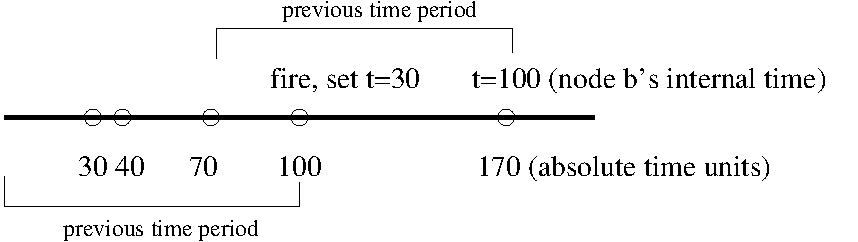
\includegraphics[width=1.0\hsize]{./figures/algo2.pdf}
%% \end{center}
%% \end{figure}


{\bf Pre-emptive Message Staggering.} CSMA schemes attempt to avoid
channel collisions by causing nodes to backoff for random intervals
prior to message transmission. The range of this random interval is
increased exponentially following each failed transmission attempt, up
to a maximum range.  If a small number of nodes are transmitting at
any point in time, then this approach induces low message delays.
However, if many nodes are transmitting simultaneously, delays may
become very large. CSMA works very well with bursty traffic and
non-uniform transmission times.  However, for the M\&S algorithm, the
communication pattern is very predictable and represents the worst
case for CSMA when many nodes are firing simultaneously.

In order to avoid repeated collisions and control the extent of
message delay, we explicitly add a random transmission delay to node
firing messages at the application level. We choose the delay
uniformly random between 0 and a constant $D$. In addition, after a
node fires, it waits for a grace period $W$ (where $W>D$ and $W \ll T$)
before processing the queue so that delayed messages from synchronized
nodes are received. In Section~\ref{sec-simulations}, we discuss our
choices for the parameter values and show that in practice this works
well to control message delay.

{\bf Simplified Firing Function.} In order to make the firing response
fast to compute, we chose a simple firing function $f(t) =
\ln(t)$. Using equation (\ref{eqn:strogatz}) along with
$f^{-1}(x)=e^x$, we can compute the jump in response to a firing
event, which is
$\Delta(t')=f^{-1}(f(t')+\epsilon)-t'=(e^{\epsilon}-1)t'$. To first
order $e^\epsilon = 1 + \epsilon$ (Taylor expansion), leaving us with
 a simple way to calculate the jump.

\begin{equation}\label{eqn:delta}
\Delta(t') = \epsilon t'
\end{equation}

%% RAD: There is no reason to invoke linearization
%% in fact we could have computed delta(t) exactly!!!
%% instead we use an approximation, which still isn't bad.
%%
%% Removed Text
%% In order make the firing response fast to compute, we chose a simple
%% firing function $f(t) = \ln(t)$ and we approximate $f(t)$ as being
%% linear over a small intervals. From equation \ref{eqn:strogatz}, we
%% know that $t'' = f^{-1}(f(t') + \epsilon)$. Assume that between time
%% $t'$ and $t''$, $f(t)$ can be approximated as a linear function $k't$
%% where $k'$ is the slope of $f$ evaluated at time $t'$. Thus $k' =
%% df/dt(t')$. Therefore, $t'' = (1/k') (k't' + \epsilon) = t' +
%% \epsilon/k' $.

%% If $f(t) = \ln(t)$, then its slope $k(t) = 1/t$, which makes the jump
%% extremely simple to compute: 

\subsection{Effect of Parameter Choices}
\label{sec:params}

The main parameter that affects the behavior of the system is
$\epsilon$, which determines the extent to which a node responds when
it observes a neighbor firing. A node responds to a neighbor by
incrementing its phase (shortening its time to fire) by $\epsilon t$,
where $t$ is the internal time at which the event was observed. Since
$t<T$, the maximum increment a node could make is $\epsilon T$. Thus
if $\epsilon = 1/100$, then a node can react to another node by at
most $T/100$. 

This gives us an intuitive feel for the effect of $\epsilon$, which is
made more concrete in the next section.  Choosing a larger epsilon
means that a node will take larger jumps in response to other nodes'
firing, thus achieving synchrony faster. However if $\epsilon$ is too
large, then nodes will ``overshoot'', preventing convergence. Making
$\epsilon$ small avoids overshooting but only at the cost of nodes
proceeding slowly towards convergence. In the next section we prove
that the time to synchronize is proportional to $1/\epsilon$, for
reasonable values of $\epsilon$. Later in the paper we present
simulation and testbed results that show that the system works well
over a wide range of $\epsilon$.


Other parameters such as the time period $T$ and the message
staggering delay $D$ do not affect the ability to converge, nor the
number of time periods to converge. The goal of $D$ is to stagger
messages within one broadcast neighborhood, therefore it should exceed
network density. The choice of $T$ affects overhead because it
represents the frequency with which nodes communicate --- one can
choose that to be appropriate for the application. The main constraint
is that $T \gg D$, so that there is enough time for all the messages
from a previous time period to be collected. In the face of heavy
congestion, this inequality may be violated in which case the delayed
firing events can simply be discarded.

For our implementation, we choose $T=1$sec and $D=25$ms. These
choices are somewhat arbitrary; our experimental results suggest that
the application layer delay of $25$ms works well to eliminate packet
loss during synchronized firings for neighborhoods of upto 20 nodes.


%% [SHOULD WE HAVE A SECTION ON IMPLEMENTATION DETAILS] In the
%% implementation of this algorithm for the nodes, the nodes do
%% additional tasks such as sort the queue, use a fixed size queue,
%% discard messages that are delayed beyond $T$ units of time, etc.
